%%%%%%%%%%%%%%%%%%%%%%%%%%%%%%%%%%%%%%%%%%%%%%%%%%%%%%%%%%%%%%%%%%%%%%%%%%%%%%%%
%%%%%%%%%%%%%%%%%%%%%%%%%%%%%%%%%%%%%%%%%%%%%%%%%%%%%%%%%%%%%%%%%%%%%%%%%%%%%%%%
\section{Activities for enlisting organizations and building support for BuB initiatives}
\label{sec:dissemination}

This section reports on the meetings attended and other activities carried out aimed at enlisting organizations and building support for BuB initiatives. It focuses on those belonging to this reporting period, but the previous ones are also listed for completeness.

%%%%%%%%%%%%%%%%%%%%%%%%%%%%%%%%%%%%%%%%%%%%%%%%%%%%%%%%%%%%%%%%%%%%%%%%%%%%%%%%
\subsection{Community Networks and BuB initiatives}

As in many other community projects, face-to-face meetings are a key component in BuB initiatives. They play a key role in strengthening relationships and the experience shows that most of the projects are debated and started in this kind of events. Thus C4EU allocated resources to attend the most relevant of these events, to present there its proposals, seeking debate and interested parties.


During the current reporting period the following events were attended:
\begin{itemize}
  \setlength{\itemindent}{2em}
  
  \item Namibia's National ICT Summit, Windhoek (Namibia), 6-7 July 2014
  \begin{itemize} \setlength{\itemindent}{2em} \item Presentation of C4EU/BuB initiative in the closing session \end{itemize}
  
  \item Participatory Networks Workshop, collocated with Participaroty Design Conference 2014 (PDC14), Windhoek (Namibia), 6-10 July 2014
  \begin{itemize} \setlength{\itemindent}{2em} \item Presentation of C4EU/BuB initiative and guifi.net project \end{itemize}
  
  \item 10th International Fab Lab Conference and Fab Festival (FAB10), Barcelona (Catalonia), 2-8 July 2014
  \begin{itemize} \setlength{\itemindent}{2em} \item Presentation of BuB tools in a plenary session \end{itemize}
  
  \item 50th Internet Corporation for Assigned Names and Numbers meeting (ICANN50) , London (UK), 22-26 June 2014
  \begin{itemize} \setlength{\itemindent}{2em} \item Private meetings \end{itemize}
  
  \item Salut, Amor i Xarxa (SAX) guifi.net meeting, Morella (Pa\'{i}s Valenci\`{a}), 7-8 June 2014
  \begin{itemize} \setlength{\itemindent}{2em} \item Presentation of the Free Network Foundation and the BuB initiative in a plenary session\end{itemize}
  
  \item Association for Progressive Communications (APC) member meeting, Barcelona (Catalonia), 1-9 June 2014
  \begin{itemize} \setlength{\itemindent}{2em} \item Presentation of the BuB initiative in a plenary session; together with the Free Network Foundation \end{itemize}
  
  \item Wireless Battle Mesh v7 (WBMv7), Leibzig (Germany), 12-18 May 2014
  \begin{itemize} \setlength{\itemindent}{2em} \item Update presentation \end{itemize}
  
  \item WIPJam@MWC214, WIPJam collocated with the Mobile World Congress, Barcelona (Catalonia), 24 February 2014
  \begin{itemize} \setlength{\itemindent}{2em} \item guifi.net invited \end{itemize}
  
  \item Barcelona The Lab, Barcelona (Catalonia), 20-21 February 2014
  \begin{itemize} \setlength{\itemindent}{2em} \item C4EU/BuB4EU presented in a working session \end{itemize}
  
  \item Free and Open Source Software Developers' European Meeting 2014 (FOSDEM14), Brussels (Belguim), 1-2 February 2014
  \begin{itemize} \setlength{\itemindent}{2em} \item Presence at the Community Networks stand. Participation in the FFDN meeting. \end{itemize}
\end{itemize}



The most relevant events where we had previously presented our initiative are:
\begin{itemize}
  \setlength{\itemindent}{2em}
  \item International Summit for Wireless Community Networks 2013, Berlin (Germany), October 2013
  \item Wireless Battle Mesh v6, Aalborg (Denmark), April 2013
  \item International Summit for Wireless Community Networks 2012, Barcelona (Catalonia), October 2012
  \item Wireless Battle Mesh v5, Athens (Greece), March 2012
\end{itemize}

\begin{itemize}
  \item International Summit for Wireless Community Networks 2012, Barcelona (Catalonia), October 2012
  \item FFTH Conference 2013, London (United Kingdom) February 2013
  \item International Summit for Wireless Community Networks 2013, Berlin (Germany), October 2013
\end{itemize}

Contacted organistaions:
\begin{itemize}
  \setlength{\itemindent}{2em}
  \item FunkFeuer, Austria
  \item Athens Wireless Metropolitan Network, Greece
  \item Sarantaporo.org, Greece
  \item Free Network Foundation, USA
  \item Altermesh, Argentina
  \item Sudo Room, USA
  \item Wlan0, Solvenia
  \item Ninux, Italy
  \item FreiFunk, Germany
\end{itemize}


%%%%%%%%%%%%%%%%%%%%%%%%%%%%%%%%%%%%%%%%%%%%%%%%%%%%%%%%%%%%%%%%%%%%%%%%%%%%%%%%
\subsection{Public administrations}

Interacting with the local governments, from city councils to the Catalan and the Spanish government is part of the standard activities of the guifi.net Foundation. Aside of those contacts that are merely formal administrative and legal proceedings (communications, notifications, etc.), the rest are aimed at creating awareness of the BuB model and at exploring forms of partnership. In most of these meetings the BuB initiative has been presented. A non-exhaustive list of public administrations we presented the initiative follows:

\begin{itemize}
  \setlength{\itemindent}{2em}
  \item City Councils: Barcelona, Sant Pere de Ribes, Sant Vicen\c{c} dels Horts, Sant Bartomeu del Grau, Manlleu, Folgueroles, Sant Juli\`{a} de vilatorta, Masies de Voltreg\`{a}, Sant Hip\'{o}lit de Voltreg\`{a}, Sallent, Calldetenes, etc.
  \item Regional governments: Consorci del Llu\c{c}\`{e}s, Consell Comarcal d'Osona, 
  \item Catalan Government: Members of the Catalan Parliament, Centre Catal\`{a} de Telecomunicacions i Tecnologies de la Informaci\'{o}(CTTI), Direcci\'{o} General de Telecomunicacions
  \item Spanish Telecommunications national regulatory authority - standard meetings kept.
\end{itemize}


%%%%%%%%%%%%%%%%%%%%%%%%%%%%%%%%%%%%%%%%%%%%%%%%%%%%%%%%%%%%%%%%%%%%%%%%%%%%%%%%
%%%%%%%%%%%%%%%%%%%%%%%%%%%%%%%%%%%%%%%%%%%%%%%%%%%%%%%%%%%%%%%%%%%%%%%%%%%%%%%%
\clearpage
\section{Tools for supporting BuB initiatives}
\label{sec:tools}

A set of tools to support BuB initiatives has been developed and integrated in guifi.net's ecosystem.

%%%%%%%%%%%%%%%%%%%%%%%%%%%%%%%%%%%%%%%%%%%%%%%%%%%%%%%%%%%%%%%%%%%%%%%%%%%%%%%%
\subsection{BuB mailing list}

Hosted at guifi.net's mailing list manager\footnote{Sympa \url{http://www.sympa.org/}.}, this public list\footnote{\url{https://llistes.guifi.net/sympa/info/bub}} was the first public mean of communication set up. Started on May 2012, as of October 2013 it had over 500 mails in total and 59 subscribers, half of them without any kind of affiliation with the Commons for Europe partners. It rapidly became the \emph{de facto} place to discuss not only about BuBforEurope but also about more general BuB issues. For instance, all project pilot's announcements, discussions, etc. have been done via this mailing list. During current reporting period it has accounted over 200 mails and the number of subscribers has increase up to 64.


%%%%%%%%%%%%%%%%%%%%%%%%%%%%%%%%%%%%%%%%%%%%%%%%%%%%%%%%%%%%%%%%%%%%%%%%%%%%%%%%
\subsection{bubforeurope.net website}

This is the reference website\footnote{\url{http://bubforeurope.net/}} for the BuB part of C4EU. During the project execution it has been used as a coordination tool for the BuB pilots as well as a gathering place for relevant BuB documentation. Now that the project is over it has been re-engineered to better suit the second goal and to merge with C4EU and codeforeurope websites look and feel. To this end a new website with less features and a clearer and lighter design has been set up, the former has been moved to another URL\footnote{\url{http://old.bubforeurope.net/}} in order to keep all its contents, and the most significant ones have been integrated with the new one. \figurename \ref{fig:bubforeurope.net} shows the front page of the new website.

\begin{figure}[H]
  \centering
  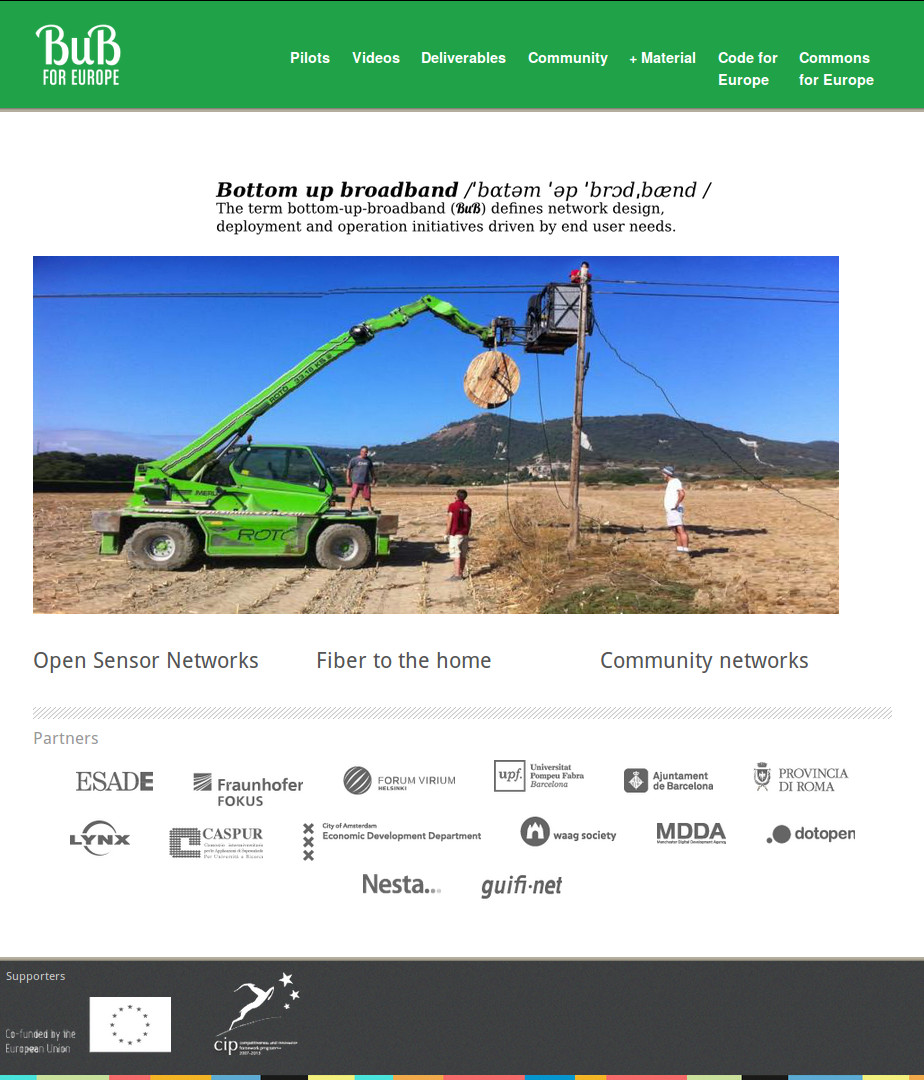
\includegraphics[width=0.95\linewidth]{sect2/figures/bubforeurope_net_crop.jpg}
  \caption[New bubforeurope.net website front page.]{New bubforeurope.net website front page.}
  \label{fig:bubforeurope.net}
\end{figure}


%%%%%%%%%%%%%%%%%%%%%%%%%%%%%%%%%%%%%%%%%%%%%%%%%%%%%%%%%%%%%%%%%%%%%%%%%%%%%%%%
\subsection{Economic compensation system}

To compensate imbalances between investment in the infrastructure held in commons and network usage among the professionals, an economic compensations system has been developed and implemented in guifi.net. Expenditures declared by the participants (professionals and volunteers) are periodically cleared according to the network usage of these professionals. Calculations are done by a third party entity, the Foundation in the guifi.net case, and are made available to the professionals. The third party centralises and manages the billing system (each professional only makes or receives a single payment). In the guifi.net case, a typical revenue for the Foundation is a percentage depending on each professional type is charged to the result of these calculations\footnote{Type A 10\% (to cover administrative costs), Type B 50\%, and Type C 100\%.}. In addition professionals are allowed to charge a reasonable amount for opportunistic connections\footnote{A client node that connects in a DiY manner to a supernode that has been paid by a professional.} until their investment is covered.

\figurename \ref{fig:comp1} shows the results of a closed period. This data is publicly available\footnote{\url{http://guifi.net/en/node/2444/view/budgets/id\%3D2444\%2Cdetails\%3Ddetailed\%2Ctypes\%3Dw-opex\%2Cstatus\%3DCompensated\%2Cfrom\%3D2014$\vert$1$\vert$1\%2Cto\%3D2014$\vert$6$\vert$30\%2Cnd\%3D\%2Corderby\%3Daccdate\%2Curl\%3Dview\%5Ebudgets} }. The screen is divided into four sections. At the top the filters section has several cells to customise the query, the section below shows the summary of the result of the query, next one shows the historic evolution of the results and the last (trimmed in the screenshot) shows each matching item, that is to say, each expenditure declared by the participants.

\begin{figure}[H]
  \centering
  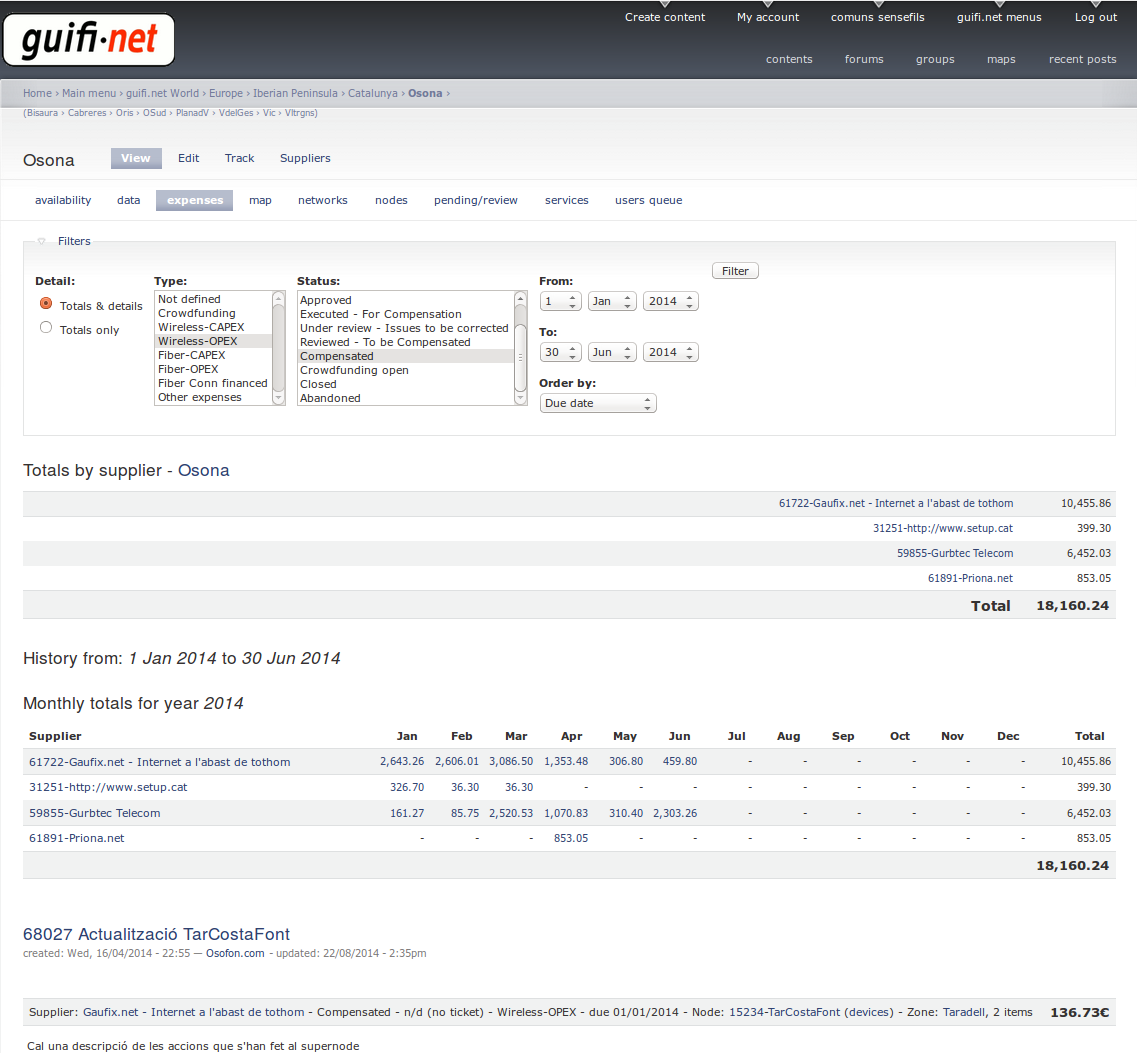
\includegraphics[width=0.95\linewidth]{sect2/figures/Compen_Osona_crop.png}
  \caption[Economic compensation system. Closed period.]{Economic compensation system. Closed period.}
  \label{fig:comp1}
\end{figure}

\figurename \ref{fig:comp2}\footnote{\url{http://guifi.net/en/node/2444/view/budgets/id\%3D2444\%2Cdetails\%3Ddetailed\%2Ctypes\%3Dw-opex\%2Cstatus\%3DReviewed\%2Cfrom\%3D2014$\vert$1$\vert$1\%2Cto\%3D2014$\vert$9$\vert$30\%2Cnd\%3D\%2Corderby\%3Daccdate\%2Curl\%3Dview\%5Ebudgets} } shows the result of another selection criterion. In this case the compensation period has not yet been closed. The rest of parameters have not been changed to allow the comparison with the results of the previous selection criterion.

\begin{figure}[H]
  \centering
  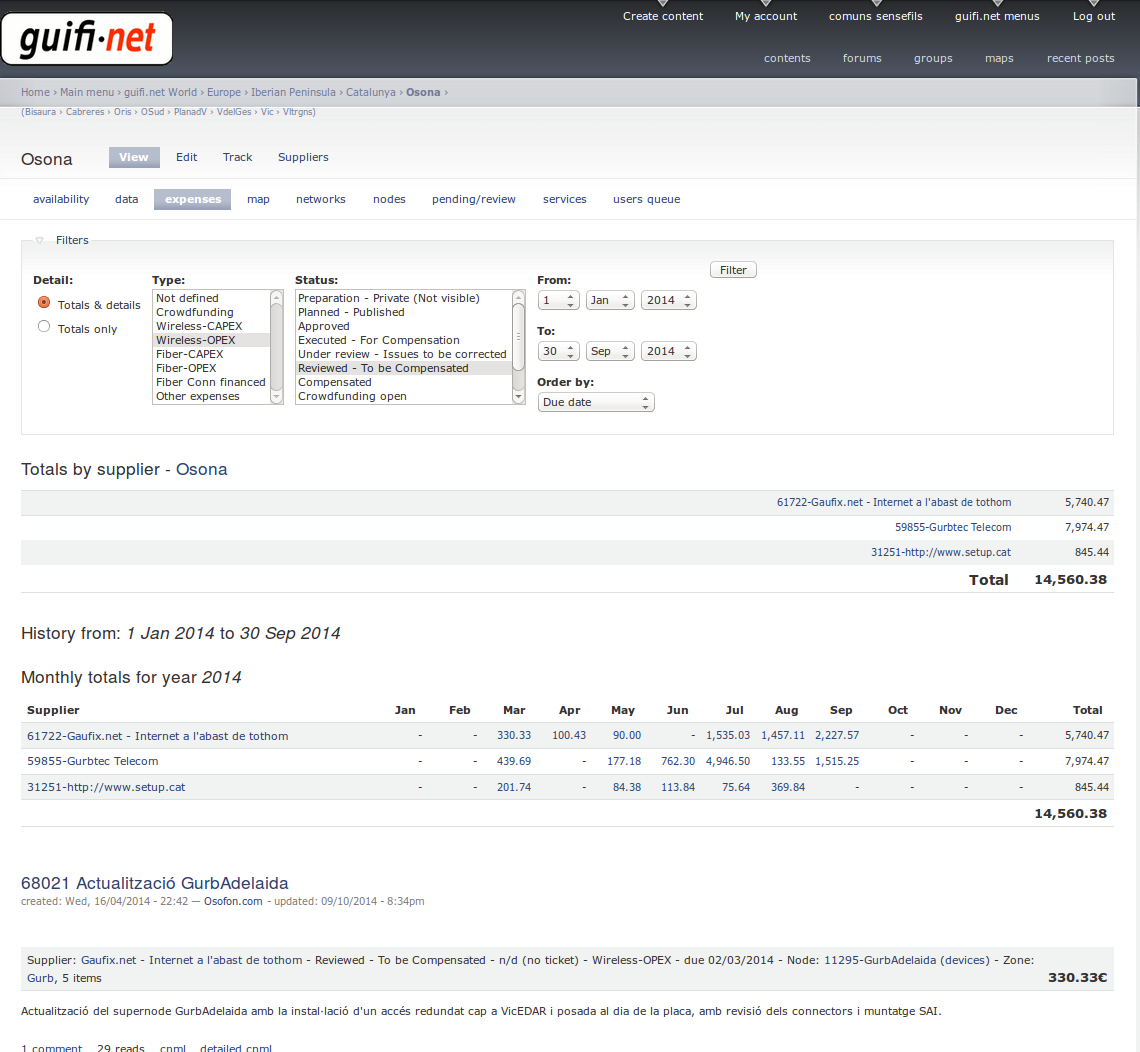
\includegraphics[width=0.95\linewidth]{sect2/figures/Compen_Osona_2_crop.png}
  \caption[Economic compensation system. Open period.]{Economic compensation system. Open period.}
  \label{fig:comp2}
\end{figure}

Finally, \figurename \ref{fig:comp3} shows the chargeback of a closed period. The total amounts of all participant are positive, that is to say, to pay, due to the recurrent costs of the Points-of-Presence, the internet uplinks, etc. but it can be observed that some of the partial values are negative, that is to say, to be reimbursed, showing that the investment made was above the consumption/usage made of the network. This information is only available to the professionals, thus, it has been appropriately anonymised.

\begin{figure}[H]
  \centering
  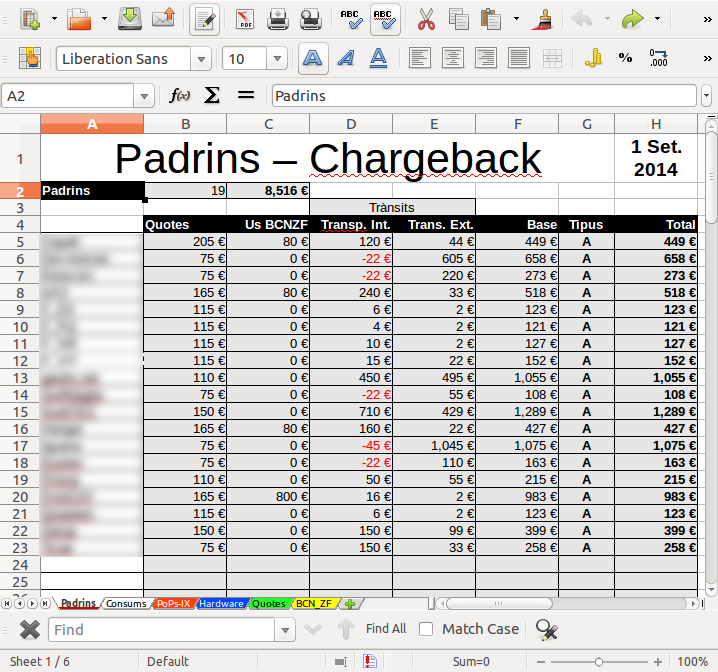
\includegraphics[width=0.65\linewidth]{sect2/figures/chargeback.png}
  \caption[Economic compensation system. Closed period.]{Chargeback of the professionals. Closed period.}
  \label{fig:comp3}
\end{figure}


%%%%%%%%%%%%%%%%%%%%%%%%%%%%%%%%%%%%%%%%%%%%%%%%%%%%%%%%%%%%%%%%%%%%%%%%%%%%%%%%
\subsection{Fiber optic web support}

The module to support and document Optic Fibre (OF) deployments was of the highest priority because OF deployments had already started long time ago but were not systematically documented due to the lack of this tool. Great efforts have been invested because to solve this problem strong modifications of the database were required and, in consequence, for many of the already existing modules as well. Nonetheless the effort has been worth because support for hybrid wireless\footnote{Hybrid wireless nodes had become the \emph{de facto} standard of Supernodes but were not yet supported either.} nodes has also been introduced\footnote{Main commit \url{https://gitorious.org/guifi/drupal-guifi/commit/f67eeff8802420cedf2eb8fc79c7d311b797c23a}}. \figurename \ref{fig:OF_sup} shows the pull-down menu of currently supported devices. It can be noticed that most of the standard OF technologies (e.g. GPON or media converters) are available.

\begin{figure}[H]
  \centering
  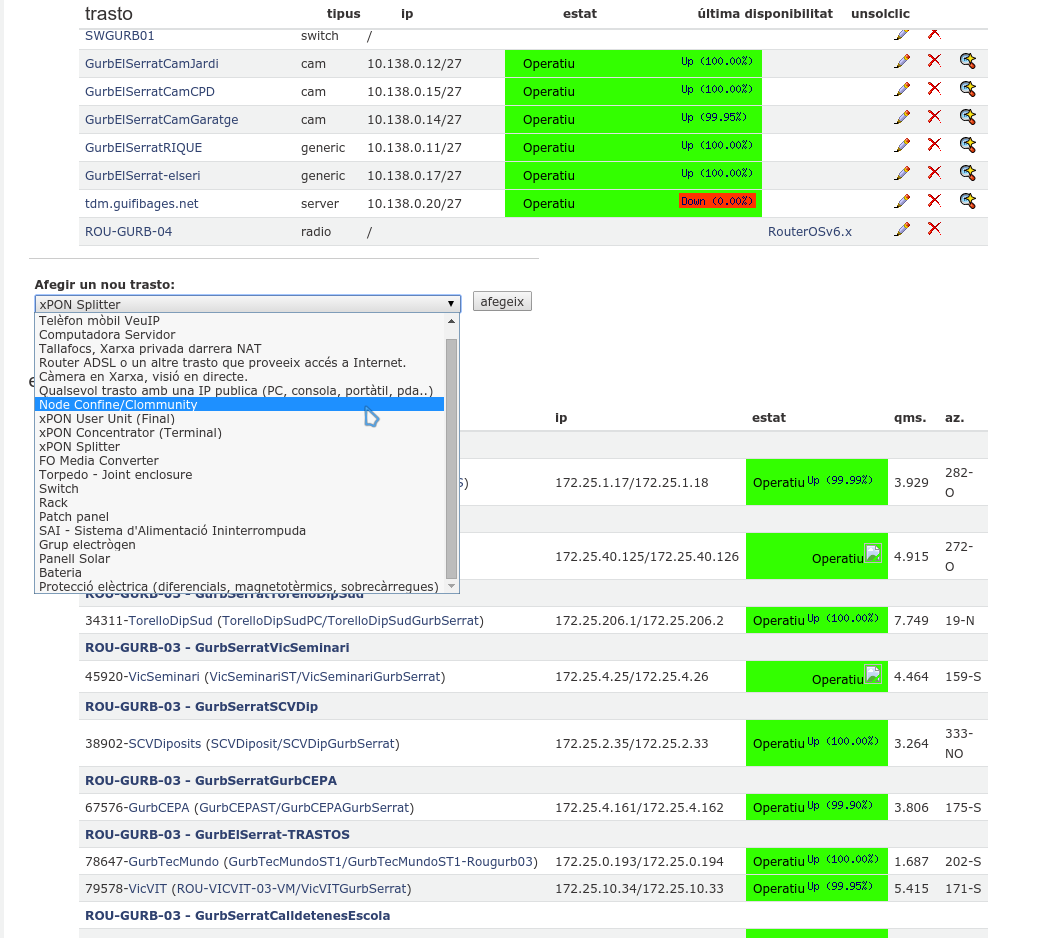
\includegraphics[width=0.95\linewidth]{sect2/figures/OF_support_crop.png}
  \caption[Fibre optic WEB module.]{Fibre optic WEB module.}
  \label{fig:OF_sup}
\end{figure}

The developed tool is now being used to document the already existing deployments such as the selected pilots of WP5.

All guifi.net source code is made publicly available through Free Software licences, the OF module inclueded.


%%%%%%%%%%%%%%%%%%%%%%%%%%%%%%%%%%%%%%%%%%%%%%%%%%%%%%%%%%%%%%%%%%%%%%%%%%%%%%%%
\subsection{Conflicts resolution procedure}

A systematic and clear procedure for resolution of conflicts with a scale of graduated sanctions has been developed\footnote{\url{http://social.guifi.net/groups/guifi-legal/reglament-dels-procediments-de-resoluci\%C3\%B3-de-conflictes}}. It consists of three stages, conciliation, mediation and arbitration, all of them driven by a lawyer chosen from a set of volunteers. The cost of the procedures are charged to the responsible part or to both parties in case of a tie. This system has defined a precise manner to address conflicts in a quick and standard way, with help from lawyers, that scales well. Its diagram flow is presented in \figurename \ref{fig:conflicts}.

\begin{figure}[H]
  \centering
  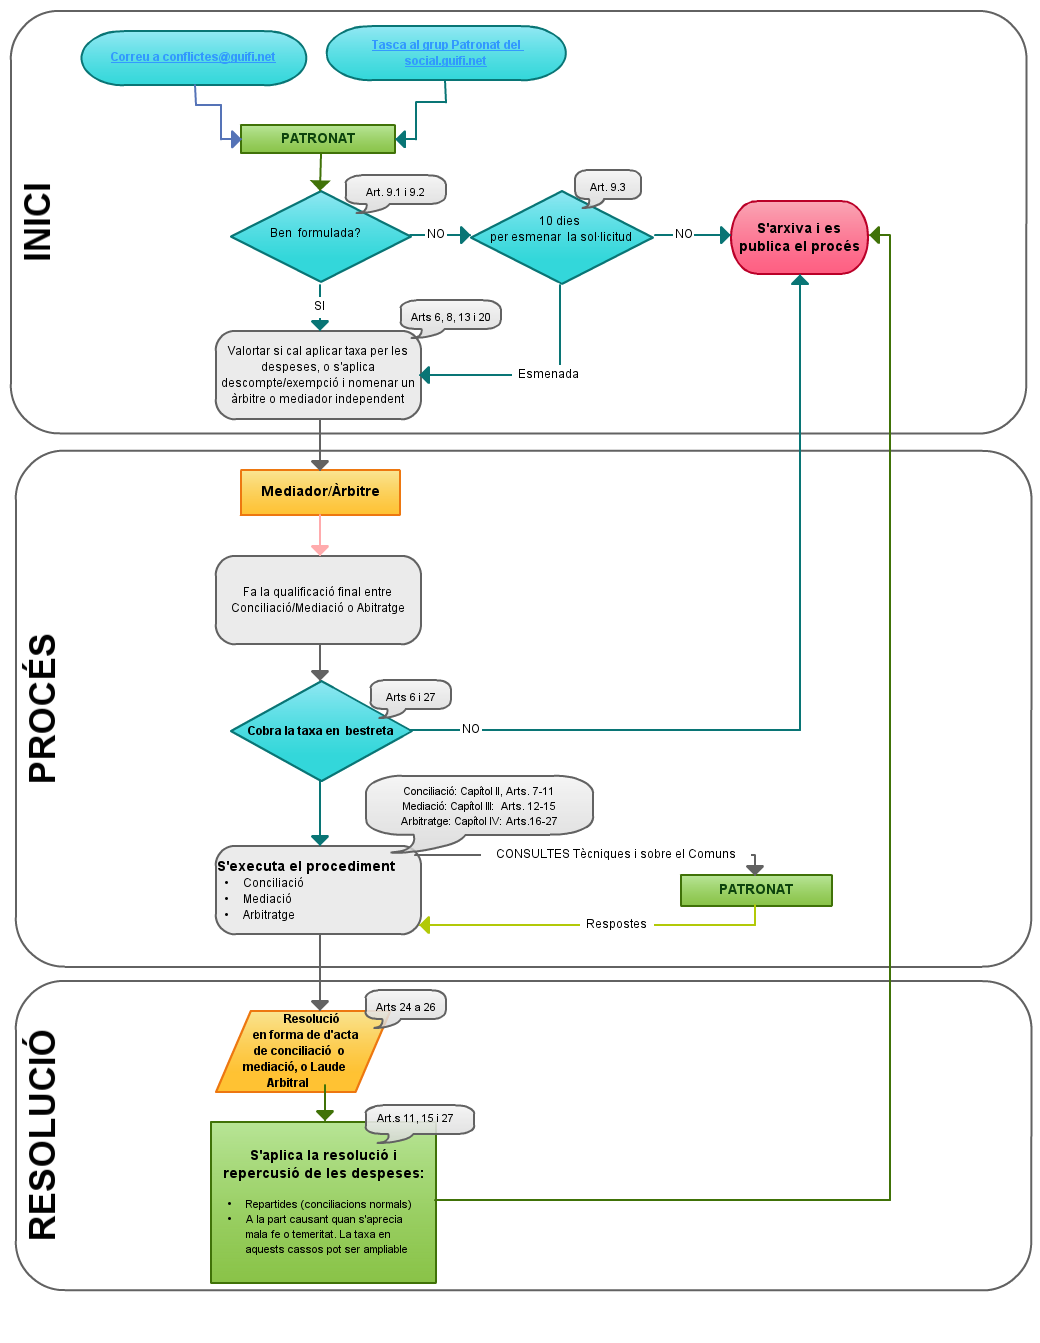
\includegraphics[width=0.90\linewidth]{sect2/figures/Resolucio_de_conflictes.png}
  \caption[Conflicts resolution system flow diagram.]{Conflicts resolution system flow diagram.}
  \label{fig:conflicts}
\end{figure}


%%%%%%%%%%%%%%%%%%%%%%%%%%%%%%%%%%%%%%%%%%%%%%%%%%%%%%%%%%%%%%%%%%%%%%%%%%%%%%%%
\subsection{The Compact for a Free, Open \& Neutral Network (FONN Compact) English translation}


NCL\footnote{\url{http://guifi.net/en/FONNC}. \textit{Llicència de Comuns per a la Xarxa Oberta, Lliure i Neutral (XOLN)} in Catalan \url{http://guifi.net/ca/CXOLN}} is the license which any guifi.net participant must subscribe. Its preamble\footnote{
FONN Compact preamble:
\begin{itemize}
  \begin{em}
    \item You have the freedom to use the network for any purpose as long as you don't harm the operation of the network itself , the rights of other users, or the principles of neutrality that allow contents and services to flow without deliberate interference.
    \item You have the right to understand the network and its components, and to share knowledge of its mechanisms and principles.
    \item You have the right to offer services and content to the network on your own terms.
    \item You have the right to join the network, and the obligation to extend this set of rights to anyone according to these same terms.
  \end{em}
\end{itemize}
}
sets the fundamental principles and the articles precisely establish the participants' rights and duties. It is written to be enforceable under the Spanish legislation. Legal certainty is essential to stimulate participation and investment, which in turn, is at the base of any economic activity. The license has been developed as part of a long lasting participatory deliberation process over several years, with contributions from many community members, reaching a consensus, revised and approved in several versions by the community assembly.

It has been identified as a key factor of guifi.net growth, thus, we considered that it should be made available to all BuB practitioners. To this end we have translated it into English (see Annex I). All guifi.net documentation, the license included, is made publicly available through free content licenses. 


%%%%%%%%%%%%%%%%%%%%%%%%%%%%%%%%%%%%%%%%%%%%%%%%%%%%%%%%%%%%%%%%%%%%%%%%%%%%%%%%
\subsection{guifi.net website English translation}

The community of guifi.net has developed a set of software tools to ease the design, deployment, management and operation of the network in a self-provisioning style and supporting crowsourced efforts by members of the community given the intrinsic inter-dependence in the computer and social network. Most of them are integrated into the guifi.net website\footnote{The guifi.net website uses Drupal as CMS and MySQL as database. All the developed tools are presented as Drupal modules.}. These tools are, along with the network license, the key tool for guifi.net growth. By participating in its translation into English we have contributed to  bring them closer to the BuB international community. \figurename \ref{fig:guifi_web} shows the guifi.net website front page in English.

\begin{figure}[H]
  \centering
  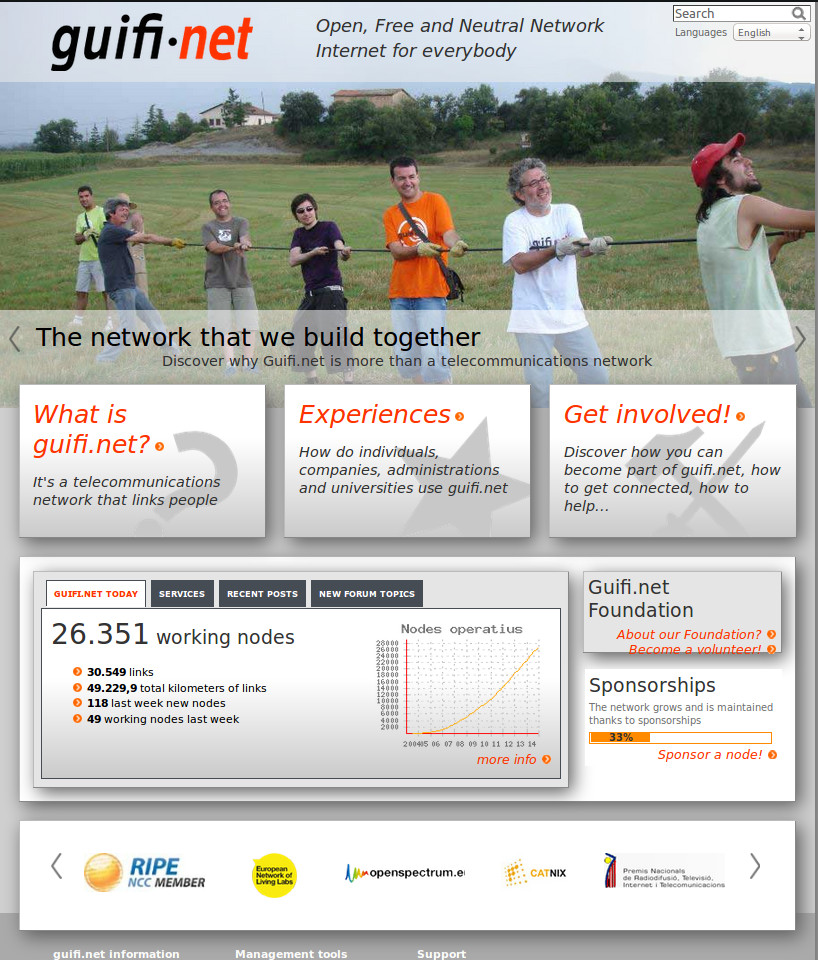
\includegraphics[width=0.75\linewidth]{sect2/figures/guifi_website_crop.jpg}
  \caption[guifi.net website front page.]{guifi.net website front page.}
  \label{fig:guifi_web}
\end{figure}

